
\begin{figure}
\begin{center}
  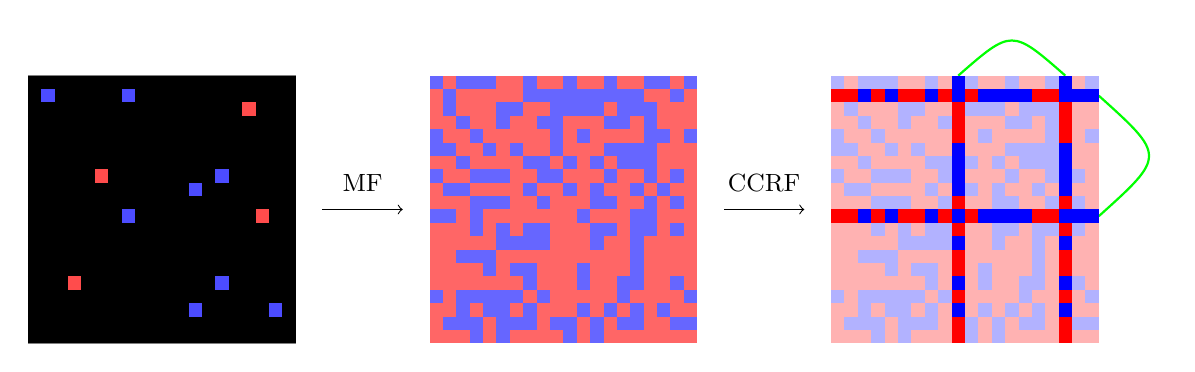
\begin{tikzpicture}[scale=0.17]
  
  \foreach \x in {0,...,19}
  	\foreach \y in {0,...,19}{
   	 \fill [red!60] (\x+30,\y) rectangle (\x+31,\y+1);
   	 \fill [red!30] (\x+60,\y) rectangle (\x+61,\y+1);
   	 }
   	 
   \foreach \x in {0,...,200}{
   	 \pgfmathsetmacro{\Xa}{random(19)}
   	 \pgfmathsetmacro{\Xb}{random(19)}
   	  \fill [blue!60] (\Xa+29,\Xb) rectangle (\Xa+30,\Xb+1);
   	  \fill [blue!60] (33,0) rectangle (34,1);
   	  \fill [blue!60] (35,0) rectangle (36,1);
   	  \fill [blue!60] (40,0) rectangle (41,1);
   	  \fill [blue!60] (42,0) rectangle (43,1);
   	  \fill [blue!60] (49,19) rectangle (50,20);
   	  \fill [blue!60] (49,15) rectangle (50,16);
   	  \fill [blue!60] (49,1) rectangle (50,2);
   	  \fill [blue!60] (49,3) rectangle (50,4);
   	  
   	  \fill [blue!30] (\Xa+59,\Xb) rectangle (\Xa+60,\Xb+1);
   	  \fill [blue!30] (63,0) rectangle (64,1);
   	  \fill [blue!30] (65,0) rectangle (66,1);
   	  \fill [blue!30] (70,0) rectangle (71,1);
   	  \fill [blue!30] (72,0) rectangle (73,1);
   	  \fill [blue!30] (79,19) rectangle (80,20);
   	  \fill [blue!30] (79,15) rectangle (80,16);
   	  \fill [blue!30] (79,1) rectangle (80,2);
   	  \fill [blue!30] (79,3) rectangle (80,4);
   	  }
   	  
   	  \draw [->] (22,10) to (28,10);
   	  
   	  \draw[help lines] (0,0) grid (20,20);
\fill [black] (0,0) rectangle (20,20);
\fill [red!70] (3,4) rectangle (4,5);
\fill [red!70] (5,12) rectangle (6,13);
\fill [blue!70] (14,12) rectangle (15,13);
\fill [red!70] (12,2) rectangle (13,3);
\fill [blue!70] (12,2) rectangle (13,3);
\fill [blue!70] (12,11) rectangle (13,12);
\fill [blue!70] (7,9) rectangle (8,10);
\fill [red!70] (17,9) rectangle (18,10);
\fill [blue!70] (7,18) rectangle (8,19);
\fill [blue!70] (1,18) rectangle (2,19);
\fill [blue!70] (18,2) rectangle (19,3);
\fill [blue!70] (14,4) rectangle (15,5);
\fill [red!70] (16,17) rectangle (17,18);

\draw [->] (52,10) to (58,10);

\draw [color=green, thick] (80,9.5) .. controls (85,14) .. (80,18.5);
\draw [color=green, thick] (69.5,20) .. controls (73.5,23.5) .. (77.5,20);
%\draw [color=green, thick] (62.5,20) .. controls (65.5,23.5) .. (68.5,20);
%\draw [color=green, thick] (80,2.5) .. controls (85,8.5) .. (80,14.5);

\foreach \x in {0,...,19}{
	\fill [red] (\x+60,18) rectangle (\x+61,19);
	\fill [red] (\x+60,9) rectangle (\x+61,10);
	%\fill [red] (\x+60,2) rectangle (\x+61,3);
	%\fill [red] (\x+60,14) rectangle (\x+61,15);
	\fill [red] (69,\x) rectangle (70,\x+1);
	\fill [red] (77,\x) rectangle (78,\x+1);
	%\fill [red] (62,\x) rectangle (63,\x+1);
	%\fill [red] (68,\x) rectangle (69,\x+1);
}
\foreach \x in {0,...,10}{
   	 \pgfmathsetmacro{\Xa}{random(19)}
   	 	\fill [blue] (\Xa+60,18) rectangle (\Xa+61,19);
   	 	\fill [blue] (\Xa+60,9) rectangle (\Xa+61,10);
   	 	
   	 	
   	 	\fill [blue] (69,\Xa) rectangle (70,\Xa+1);
   	 	\fill [blue] (77,\Xa) rectangle (78,\Xa+1);
   	}
   	
   	\node at(55,12){\small CCRF};
   	\node at(25,12){\small MF};
	\end{tikzpicture} 

	\end{center}
	\caption{First, Matrix Factorization is applied to get an initial prediction, then a graphical model (CCRF) is utilized to introduce similarity matrices of the drugs and targets.}
	\label{fig:pipeline}
	\end{figure}